\section{Widget}
\label{chap:widget}
\begin{figure}[h]
\centering
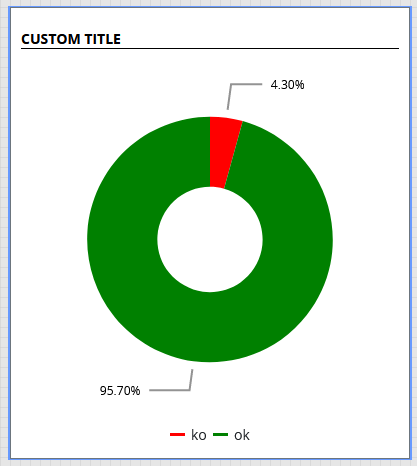
\includegraphics[scale=0.6]{images/widget_example.png}
\end{figure}
\subsection{Composizione}

Un \textit{widget} è una piccola applicazione, semplice e immediata, che mostra all'utente dati e informazioni, di solito sotto forma di grafici o tabelle. \newline Prendendo ad esempio il \textit{pie chart} widget si può vedere come un widget lato \textit{frontend} sia formato da diversi \textit{file}. La classe contenente i parametri volti alla visualizzazione grafica del widget si chiama \textit{PieChartWidget}. Estende la classe \textit{BaseWidget}, dove viene gestita tutta la logica per la presa dei dati dal \textit{backend}, ed è decorata con il \textit{WidgetDecorator}, il quale aggiunge ulteriore comportamento al widget.

\begin{lstlisting}[caption={Classe PieChartWidget}, style=javaScriptCode]
@WidgetDecorator({
    endpoint: 'tuple',
    type: WidgetTypeEnum.MOBILITY,
    sourceable: true,
    adapter: PieChartAdapter,
    refreshableInfo: {
        refreshable: true,
    }
})
export class PieChartWidget extends BaseWidget {

    private titleParameter: StringParameter;

    constructor(injector: Injector, widgetDescriptor: WidgetDescriptor) {
        super(injector, widgetDescriptor);
        this.setSize(420, 450);
    }

    public get title(): string {
        return this.titleParameter.value;
    }

    protected createConfigParameters(): Observable<Parameter<unknown>[]> {
        this.createTitleParameter();
        return super.createConfigParameters();
    }

    private createTitleParameter() {
        this.titleParameter = new StringParameter('title', 'Title', 'My title');
        this.titleParameter.longText = 'Title Color';
        this.configParameters.push(this.titleParameter);
    }
}

\end{lstlisting}
Tutta la logica riguardante la visualizzazione dei dati del widget si trova nella classe \textit{PieChartComponent}. Al suo interno viene specificato come la \textit{label} debba essere mostrata nel pie chart (con il metodo \textit{labelContent}) e viene implementato il metodo \textit{getDataCallback}, richiesto dalla classe \textit{BaseWidgetComponent} che viene estesa da \textit{PieChartComponent}, per salvarsi i dati ogni qualvolta il widget riceva dati dal backend.

\begin{lstlisting}[caption={Classe PieChartComponent}, style=javaScriptCode]
@Component({
    selector: 'app-pie-chart-widget',
    templateUrl: './pie-chart.component.html',
    encapsulation: ViewEncapsulation.None,
    changeDetection: ChangeDetectionStrategy.OnPush
})
export class PieChartComponent extends BaseWidgetComponent<PieChartWidget> {

    public data: TupleData[] = [];
    public backgroundColor = '#ffffff';

    constructor(widgetActions: WidgetActions, injector: Injector) {
        super(widgetActions, injector);
        this.labelContent = this.labelContent.bind(this);
    }

    public labelContent(args: LegendLabelsContentArgs): string {
        return `${args.dataItem.value.toFixed(2)}%`;
    }

    protected getDataCallback(value: any): void {
        this.data = value;
    }
}
\end{lstlisting}
Nel file HTML, di cui viene passato il path al \textit{Component} \textit{decorator}, viene specificato l'aspetto grafico che avrà il widget all'interno della \textit{dashboard}.

\begin{lstlisting}[caption={File pie-chart.component.html}, style=javaScriptCode]
<aulos-widget-layout [widget]="widget" [backgroundColor]="backgroundColor">
    <aulos-widget-title>
        {{ widget.title }}
    </aulos-widget-title>
    <aulos-widget-content>
        <kendo-chart #customChart [chartArea]="{opacity: 0}">
            <kendo-chart-legend position="bottom"></kendo-chart-legend>
            <kendo-chart-series>
                <kendo-chart-series-item type="donut" [data]="data" field="value" 
                        categoryField="label" colorField="color">
                    <kendo-chart-series-item-labels position="outsideEnd" color="#000" 
                            background="#FFFFFF" [content]="labelContent">
                    </kendo-chart-series-item-labels>
                </kendo-chart-series-item>
            </kendo-chart-series>
        </kendo-chart>
    </aulos-widget-content>
</aulos-widget-layout>
\end{lstlisting}
Infine ogni widget viene incluso in un modulo Angular. All'avvio dell'applicazione il widget viene registrato nel sistema con la chiamata del metodo \textit{registerWidgets}, presente nel modulo. Ciò permette ad AULOS di inserirlo nella lista di widget instanziabili nella dashboard.

\begin{lstlisting}[caption={Metodo all'interno del modulo che registra il widget nel sistema}, style=javaScriptCode]
private static registerWidgets(widgetsService: WidgetComponentsService): () => 
    Promise<any> {
        const result = (): Promise<any> => {
            return new Promise((resolve, reject) => {
                const myWidgetDescriptor: WidgetDescriptor = {
                    code: 'pieChartWidgetCode',
                    shortText: 'Pie Chart',
                    longText: 'Descrizione',
                    icon: 'fa fa-pie-chart',
                    group: 'Mobility Group'
                };
                widgetsService.register(myWidgetDescriptor, PieChartWidget, 
                    PieChartComponent);

                resolve();
            });
        };
        return result;
    }
\end{lstlisting}

\subsection{Le classi BaseWidget e BaseWidgetComponent}
\label{subsec:base}
Le classi \textit{BaseWidget} e \textit{BaseWidgetComponent} sono state create con l'obiettivo di alleggerire il carico di lavoro inerente allo sviluppo di un widget. In esse risiede tutta la logica di interfacciamento con il backend, lasciando come unica responsabilità alle classi che le estendono le modalità attraverso le quali vengono visualizzati i dati.
\\
\textit{BaseWidget} e \textit{BaseWidgetComponent} estendono rispettivamente le classi, già presenti nel framework AULOS, \textit{Widget} e \textit{WidgetComponent}.
\\
All'interno del \textit{BaseWidget} viene iniettato e utilizzato il \textit{WidgetService}, servizio in cui avvengono le chiamate REST, e vengono creati i parametri \textit{source} e \textit{filters}. 

\begin{lstlisting}[caption={Creazione dei parametri all'interno della classe BaseWidget}, style=javaScriptCode]
export class BaseWidget extends Widget {

    ...

    private createSourceParameter() {
        this.sourceParameter = new StringParameter('source', 'Source', '');
        this.sourceParameter.longText = 'Source';
        this.sourceParameter.descriptor.editor = new EditorDescriptor(EDITOR_BASE_PATH,
            'SourceEditor');
    }

    private createFiltersParameter() {
        this.filtersParameter = new ContainerParameter('filters', 'Filters', null);
        this.configParameters.push(this.filtersParameter);
    }

}
\end{lstlisting}

Il parametro \textit{source} indica da quale contesto verranno presi i dati da visualizzare, mentre il parametro \textit{filters} contiene tutti i parametri che aggiungono filtri in fase di ottenimento dati (e.g. un intervallo di tempo per il quale si vogliono ottenere i risultati di un test). Il tutto viene inizializzato e caricato tramite il metodo \textit{initSourceCalls}.

\begin{lstlisting}[caption={Inizializzazione dei parametri all'interno della classe BaseWidget}, style=javaScriptCode]
export class BaseWidget extends Widget {
    
    ...
    
    private async initSourceCalls() {
        this.filtersParameter.stateChanges.subscribe(_ => {
            if (this.filtersSet && !this.widgetDTO) {
                this.getData();
            }
        });

        await this.sourceParameter.valueChanges.subscribe(sourceCode => {
            this.sourceSet = true;
            this.widgetService.getSourceProperties(sourceCode).subscribe
            (sourceProperties => {
                this.metadata = sourceProperties.metadata;
                this.setFilters(sourceProperties.filters);
                this.notifyStateChanged();
            });
        });
        this.initSource();
    }

    private getData() {
        if (!this.sourceParameter.value) { return; }
        if (!this.isFiltersReady()) { return; }
        this.widgetService.getData(this.endpoint, this.createRequest()).subscribe
            (value => {
                const data = MetadataService.map(value, this.metadata);
                this.widgetDataSubject.next(data);
        });
    }

    private initSource() {
        this.widgetService.getSource(this.endpoint).subscribe(sourceCode => {
            this.sourceParameter.value = sourceCode;
            this.sourceSet = true;
        });
    }

}
\end{lstlisting}
Nel \textit{BaseWidgetComponent} vi è la sottoscrizione al \textit{dataObservable}, attributo \textit{Observable} fornito da \textit{BaseWidget}, la quale si occupa di chiamare il metodo \textit{getDataCallback} ogni qualvolta vengono presi dati dal backend.
\begin{lstlisting}[caption={Metodi per l'inizializzazione dei dati all'interno della classe BaseWidgetComponent}, style=javaScriptCode]
@Directive()
export abstract class BaseWidgetComponent<T extends BaseWidget> extends 
    WidgetComponent<T> implements OnInit, OnDestroy{

    ...
        
    private initData() {
        this.widget.dataObservable.subscribe(value => {
            if (!value)
                {return;}
            this.getDataCallback(value);
            this.loading = false;
            this.changeDetectorRef.markForCheck();
        });
    }

    protected abstract getDataCallback(value: any): void;
}
\end{lstlisting}

\subsection{Il servizio WidgetService}
Nel \textit{WidgetService} avviene tutta la comunicazione tra frontend e backend.
La sua responsabilità è quella di fare chiamate REST per ottenere i dati da far visualizzare all'interno dei widget. Il principale metodo che si occupa di fare ciò è il metodo \textit{getData} il quale, passatagli una \textit{GenericRequest} composta da un \textit{sourceCode} e un \textit{array} di filtri, manda una richiesta POST al backend.

\begin{lstlisting}[caption={Metodo getData all'interno della classe WidgetService}, style=javaScriptCode]
@Injectable({
    providedIn: 'root'
})
export class WidgetService {

    ...

    public getData(widgetUrl: string, genericRequest: GenericRequest, adapt?: (any) => any): Observable<unknown[]> {
        const restCall = this.http.post<unknown[]>(`${this.widgetsUrl}/${widgetUrl}`, genericRequest);
        return adapt ? restCall.pipe(map((data) => adapt(data))) : restCall;
    }
    
    ...

}

\end{lstlisting}
Se il widget ha associata una funzione \textit{adapt}, questa verrà passata al metodo \textit{getData} il quale la userà per adattare i dati prima di restituirli. In caso contrario verranno passati al widget i dati nella forma in cui sono al momento della risoluzione della chiamata REST.

La lista di \textit{source} disponibili e la possibile lista di filtri e metadati si ricavano rispettivamente dal metodo \textit{getSources} e dal metodo \textit{getSourceProperties}.

\begin{lstlisting}[caption={Metodi getSources e getSourceProperties all'interno della classe WidgetService}, style=javaScriptCode]
@Injectable({
    providedIn: 'root'
})
export class WidgetService {

    ...
        
    public getSources(widgetUrl: string): Observable<SourceInfo[]> {
        return this.http.get<SourceInfo[]>(`${this.apiUrl}/${widgetUrl}/discovery`);
    }

    public getSourceProperties(sourceCode: string): Observable<SourceProperties> {
        return this.http.get<SourceProperties>(`${this.apiUrl}/filters/${sourceCode}`);
    }

}
\end{lstlisting}
Se un widget è di tipo \textit{MOBILITY}, ovvero legato a dei dati provenienti dalle macchine Loccioni, avrà bisogno della possibilità di filtrare i dati in base a \textit{linea}, \textit{banco} e \textit{stazione}. Per questo all'interno del \textit{WidgetService} vi sono tre metodi predisposti per il recupero di questi ultimi.

\begin{lstlisting}[caption={Metodi per recuperare linee, banchi e stazioni all'interno della classe WidgetService}, style=javaScriptCode]
@Injectable({
    providedIn: 'root'
})
export class WidgetService {

    ...
        
    public getLines(sourceCode: string): Observable<number[]> 
    {
        return this.http.get<number[]>(`${this.apiUrl}/topology/${sourceCode}
            /lines`);
    }

    public getBenches(sourceCode: string, lineCode: number): Observable<number[]> 
    {
        return this.http.get<number[]>(`${this.apiUrl}/topology/${sourceCode}
            /benches/${lineCode}`);
    }

    public getStations(sourceCode: string, stationCode: number): Observable<number[]> 
    {
        return this.http.get<number[]>(`${this.apiUrl}/topology/${sourceCode}
            /stations/${stationCode}`);
    }

}
\end{lstlisting}

\subsection{Il decorator factory WidgetDecorator}
\label{subsec:widgetDecorator}
Il \textit{WidgetDecorator} ha la responsabilità di aggiungere comportamento a un widget in base alle opzioni passate con l'interfaccia \textit{WidgetOptions}.

\textit{WidgetOptions} ha la seguente struttura:

\begin{lstlisting}[caption={Struttura delle WidgetOptions e delle RefreshableInfo}, style=javaScriptCode]
export interface WidgetOptions {
    // indicates which endpoint the widget has to use to take data from
    endpoint: string;
    // indicates the widget type (currently IT/MOBILITY)
    type: WidgetTypeEnum;
    // indicates whether or not the widget has a selectable source parameter
    sourceable?: boolean;
    /* indicates whether or not the widget has a refresh parameter and can be 
    used to set the default refresh rate*/
    refreshableInfo?: RefreshableInfo; 
    /* indicates the adapter class used to transform received data into a 
    more useful form*/
    adapter?: any;
}

export interface RefreshableInfo {
    refreshable: boolean;
    defaultRefreshRate?: RefreshRateEnum;
}
\end{lstlisting}
Il comportamento viene aggiunto al widget tramite altri decorator verificando le opzioni passate al momento della decorazione.

\begin{lstlisting}[caption={Decorator factory WidgetDecorator}, style=javaScriptCode]
export const WidgetDecorator: (options: WidgetOptions) => (target: Function) => 
    void = (options: WidgetOptions) => {

    return (target: Function) => {
        target.prototype.baseWidgetDecorator = true;
        target.prototype.endpoint = options.endpoint;

        switch (options.type) {
            case WidgetTypeEnum.IT:
                break;
            case WidgetTypeEnum.MOBILITY:
                Mobility(target);
                break;
        }
        if (options.sourceable) {
            Sourceable(target);
        }
        if (options.refreshableInfo?.refreshable) {
            Refreshable({defaultRefreshRate: options.refreshableInfo
                .defaultRefreshRate})(target);
        }

        if (options.adapter) {
            const adaptFunc = options.adapter.prototype.adapt;
            if (adaptFunc) {
                Adapters.setAdapter(target.prototype.endpoint, adaptFunc);
            }
        }
    };
};
\end{lstlisting}
\subsection{Mobility Decorator}
Il \textit{Mobility} decorator si occupa di aggiungere i parametri atti al filtraggio dei dati di un widget in base a linea, banco e stazione.

\begin{lstlisting}[caption={Metodo di creazione dei parametri all'interno del decorator Mobility}, style=javaScriptCode]
export const Mobility: (target: Function) => void = (target: Function) => {

    ...

    target.prototype.createTopologyParameters = function(...args) {
        target.prototype.lineCodeParameter = new NumberParameter('lineCode', 
            'Line Code', 0);
        target.prototype.benchCodeParameter = new NumberParameter('benchCode', 
            'Bench Code', 0);
        target.prototype.stationCodeParameter = new NumberParameter('stationCode', 
            'Station Code', 0);

        this.lineCodeParameter.descriptor.editor = new EditorDescriptor(
            EDITOR_BASE_PATH, 'DropdownEditor', []);
        this.benchCodeParameter.descriptor.editor = new EditorDescriptor(
            EDITOR_BASE_PATH, 'DropdownEditor', []);
        this.stationCodeParameter.descriptor.editor = new EditorDescriptor(
            EDITOR_BASE_PATH, 'DropdownEditor', []);

        this.configParameters.push(this.lineCodeParameter);
        this.configParameters.push(this.benchCodeParameter);
        this.configParameters.push(this.stationCodeParameter);
    };

};
\end{lstlisting}
Il metodo che inizializza e definisce il comportamento che il widget avrà al cambio di uno dei parametri è il metodo \textit{initTopology}.

\begin{lstlisting}[caption={Metodo initTopology all'interno del decorator Mobility}, style=javaScriptCode]
export const Mobility: (target: Function) => void = (target: Function) => {

    ...

    target.prototype.initTopology = function(...args) {
        if (this.sourceSet) {
            this.getLines(this.sourceParameter.value, this);
        }
        this.sourceParameter.valueChanges.subscribe(sourceCode => {
            this.getLines(sourceCode, this);
        });

        this.lineCodeParameter.valueChanges.subscribe(lineCode => {
            this.resetBench(this);
            this.getData(this);
            if (this.sourceParameter.value) {
                this.widgetService.getBenches(this.sourceParameter.value, lineCode)
                    .subscribe(benchCodes => {
                    this.benchCodes = benchCodes;
                    this.benchCodeParameter.descriptor.editor.options = benchCodes;
                    this.benchCodeParameter.notifyStateChanged();
                });
            }
        });

        this.benchCodeParameter.valueChanges.subscribe(benchCode => {
            this.resetStation(this);
            this.getData(this);
            if (this.sourceParameter.value) {
                this.widgetService.getStations(this.sourceParameter.value, benchCode)
                    .subscribe(stationCodes => {
                    this.stationCodes = stationCodes;
                    this.stationCodeParameter.descriptor.editor.options = stationCodes;
                    this.stationCodeParameter.notifyStateChanged();
                });
            }
        });

        this.stationCodeParameter.valueChanges.subscribe(_ => {
            this.getData(this);
        });
    };

};
\end{lstlisting}

\subsection{Sourceable decorator}
Il \textit{Sourceable} decorator dà al widget la possiblità di far selezionare all'utente la source dove prendere i dati dal backend.

Ogni widget che estende \textit{BaseWidget} ha al suo interno il parametro \textit{SourceParame}-\textit{ter}. Nel \textit{baseWidget} \textit{initSource} si occupa di impostare l'unica source da cui il widget prenderà i dati, mentre con l'override all'interno del \textit{Sourceable} decorator il metodo ha lo scopo di impostare la source in base a ciò che selezionerà l'utente.

\begin{lstlisting}[caption={Metodo initSource e override}, style=javaScriptCode]
export class BaseWidget extends Widget {
    
    ...
    
    private initSource() {
        this.widgetService.getSource(this.endpoint).subscribe(sourceCode => {
            this.sourceParameter.value = sourceCode;
            this.sourceSet = true;
        });
    }
    
}


export const Sourceable = (target: Function) => {

    ...

    target.prototype.initSource = function() {
        this.sourceParameter.valueChanges.subscribe(sourceCode => {
            this.sourceParameter.value = sourceCode;
        });
    };

};
\end{lstlisting}
La configurazione delle possibili source disponibili avviene nell'override del metodo \textit{initSourceCalls}. Le \textit{options} per l'\textit{editor} del \textit{sourceParameter} vengono impostate con il metodo \textit{setSources}.

\begin{lstlisting}[caption={Metodo setSources e override del metodo initSourceCalls all'interno del Sourceable Decorator}, style=javaScriptCode]
export const Sourceable = (target: Function) => {

    ...
    
    const oldInitSourceCalls = target.prototype.initSourceCalls;
    target.prototype.initSourceCalls = function() {
        this.widgetService.getSources(target.prototype.endpoint).subscribe(sources => {
            this.setSources(sources);
        });
        if (oldInitSourceCalls){
            oldInitSourceCalls.apply(this);
        }
    };

    target.prototype.setSources = function(sources: SourceInfo[]) {
        this.sourceParameter.descriptor.editor.options = sources;
    };

};
\end{lstlisting}
\subsection{Refreshable decorator}
Il \textit{Refreshable} decorator permette al widget di aggiornarsi e ricaricare i dati nell'arco di uno specifico intervallo di tempo. Il valore di default dell'intervallo può essere cambiato passando all'interno delle \textit{RefreshableInfo} anche un \textit{defaultRefreshRate}.
L'intervallo poi potrà essere selezionato dall'utente al momento di configurazione della dashboard grazie al \textit{refreshRateParameter} che viene aggiunto al widget.

\begin{lstlisting}[caption={Creazione del refreshRateParameter all'interno del Refreshable decorator}, style=javaScriptCode]
export const Refreshable: (options?: RefreshableOptions) => (Function) => 
    void = (options?: RefreshableOptions) => {
    return (target: Function) => {
        
        ...
        
        target.prototype.createRefreshParameter = function() {
            target.prototype.refreshRateParameter = new NumberParameter('refreshRate', 
                'Refresh Rate', this.defaultRefreshRate);
            this.refreshRateParameter.descriptor.editor = new EditorDescriptor(
                EDITOR_BASE_PATH,
                'EnumEditor',
                this.generateDefaultEnumOptions());
            this.configParameters.push(this.refreshRateParameter);
        };
        
    };
};
\end{lstlisting}
Ogni qualvolta un utente cambi intervallo di \textit{refresh} viene effettuata una nuova registrazione all'\textit{Observable} presente nel \textit{RefreshService}, legato a quel determinato intervallo, e viene annullata la precedente registrazione.

\begin{lstlisting}[caption={Metodo updateSubscription all'interno del Refreshable decorator}, style=javaScriptCode]
export const Refreshable: (options?: RefreshableOptions) => (Function) => 
    void = (options?: RefreshableOptions) => {
    return (target: Function) => {
        
        ...

        target.prototype.updateSubscription = function(refreshRate: number) {
            if (this.subscription) { this.subscription.unsubscribe(); }
            this.subscription = this.refreshService.getObservableOfInterval(refreshRate)
                .pipe(
                    exhaustMap(() => { this.getData(); return EMPTY; })
                )
                .subscribe();
        };
        
    };
};
\end{lstlisting}
Il \textit{RefreshService} ha la responsabilità di tenere salvati gli \textit{Observable} legati a tutti gli intervalli richiesti.

\begin{lstlisting}[caption={Classe RefreshService}, style=javaScriptCode]
@Injectable({
  providedIn: 'root'
})
export class RefreshService {

  private intervals: Map<number, Observable<any>> = new Map();
  constructor() { }

  public getObservableOfInterval(refreshRate: number): Observable<any> {
    if (!this.intervals.has(refreshRate)) {
      this.intervals.set(refreshRate, interval(refreshRate).pipe(
        multicast(new Subject()),
        refCount()
      ));
    }
    return this.intervals.get(refreshRate);
  }
}
\end{lstlisting}
Nello specifico il metodo \textit{getObservableOfInterval} ritorna l'\textit{Observable} dell'intervallo di tempo fornito. Se l'intervallo non è presente all'interno di \textit{intervals} allora lo inserisce creando l'\textit{Observable} legato ad esso.

L'\textit{Observable} viene creato con il metodo \textit{interval}, il quale crea un \textit{Observable} che emette numeri sequenziali all'intervallo di un tempo specificato. Poi viene trasformato con il metodo \textit{multicast} in un \textit{ConnectableObservable}, particolare tipo di \textit{Observable} che non emetterà valori finché non sarà chiamato il metodo \textit{connect}. Questa chiamata viene resa automatizzata grazie al metodo \textit{refCount}, il quale gestisce la connessione in modo tale da mantenerla attiva fintanto che ci siano \textit{observer} in ascolto.

\begin{lstlisting}[caption={Classe RefreshService}, style=html]
<aulos-editor-layout [editorConfiguration]="editorConfiguration">
  <ng-template aulosEditorSmallTemplate>
    <div class="input-group" [class.hidden]="disabled">
      <input type="text" 
        class="form-control form-control-sm is-invalid"
        [placeholder]=mySelection[0] ? mySelection[0] : 
        'Choose data source...'  | aulosTranslate 
        disabled readonly>
      <button class="btn btn-sm btn-icon" [disabled]="disabled" (click)="showExpandedModal()">
        <i class="fontaulos fontaulos-edit"></i>
      </button>
    </div>
  </ng-template>
  <ng-template aulosEditorCompactTemplate>
    <div class="input-group" [class.hidden]="disabled">
      <input 
      type="text" 
      class="form-control is-invalid" 
      [placeholder]="this.model.value ? 
      this.model.value : 
      'Choose data source...'  | aulosTranslate" 
      disabled
        readonly>
      <button class="btn btn-icon" [disabled]="disabled" (click)="showExpandedModal()">
        <i class="fontaulos fontaulos-edit"></i>
      </button>
    </div>
  </ng-template>
  <ng-template aulosEditorExpandedTemplate>
    <kendo-grid
              [data]="gridData"
              [style.maxlength]="501"
              [filterable]="true"
              [filter]="state.filter"
              [selectable]="selectableSettings"
              [sortable]="true"
              style="padding-top: 2%; padding-bottom: 5%;"
              (dataStateChange)="dataStateChange($event)"
              kendoGridSelectBy="sourceCode"
              [selectedKeys]="tmpSelection"
            >
            <kendo-grid-checkbox-column width="60%"></kendo-grid-checkbox-column>
            <kendo-grid-column field="sourceCode" filter="text"></kendo-grid-column>
            <kendo-grid-column field="shortText" filter="text"></kendo-grid-column>
            <kendo-grid-column field="longText" filter="text"></kendo-grid-column>
            <ng-template kendoGridNoRecordsTemplate>
              No sources available.
           </ng-template>
          </kendo-grid>
  </ng-template>
</aulos-editor-layout>
\end{lstlisting}